\section{Online monitoring}

The model just built is now ready to be used to classify the upcoming tweets. Predictive modeling consists in learning a model from historical data and using the model to make predictions on new data where the answer is unknown. For this reason, it is possible that a model built on past data can not be suitable for the analysis of subsequent data.

It is well known from the literature that classification models for analyzing streams of data suffer from \textbf{concept drift}. In predictive analytics and machine learning, the concept drift means that the statistical properties of the target variable, which the model is trying to predict, change over time in unexpected ways. This causes problems because predictions may become less accurate as time goes on.

For what concern text mining this problem occurs because people may change the way they express their ideas on social medias according to real world events. The consequence is that the volume of the data collected can be different and the features may change. 
If these changes are able to be detected, it may be possible to update the learned model to avoid performance loss. 

\subsection{Identifying peaks}

In order to understand if the ComplementNB model, built in the previous phases, suffers from concept drift, some {peaks},  probably corresponding to some events verified immediately before, have been identified from the overall distribution of the collected tweets  in the period following the test (Figure \ref{online-monitoring}). 

The goal is to analyze the behaviour of the built model during the days associated with the occur of some  events. Indeed, during these days, a change of the terminology used is expected and, for this reason, the corresponding tweets are particularly useful to highlight the concept drift. 
The objective of this analysis is to adapt the vocabulary used by the model in order to find a way to alleviate the concept drift.

The days highlighted in the diagram in Figure \ref{online-monitoring} correspond to the peaks chosen for the experiments conducted on the concept drift. \textbf{80 tweets} were randomly selected from every peak, except for the last peak for which were selected only \textbf{60 tweets} because the number of tweets decreases. Moreover, since no relevant peaks were found in May, 80 tweets were randomly taken from the entire month.
The peak corresponding to the 1st of March has been discarded because too close to the test set: in a more central date with respect to the month, as 2022-03-10, the effects of concept drift may be more evident.

\begin{figure}[H]
    \centering
    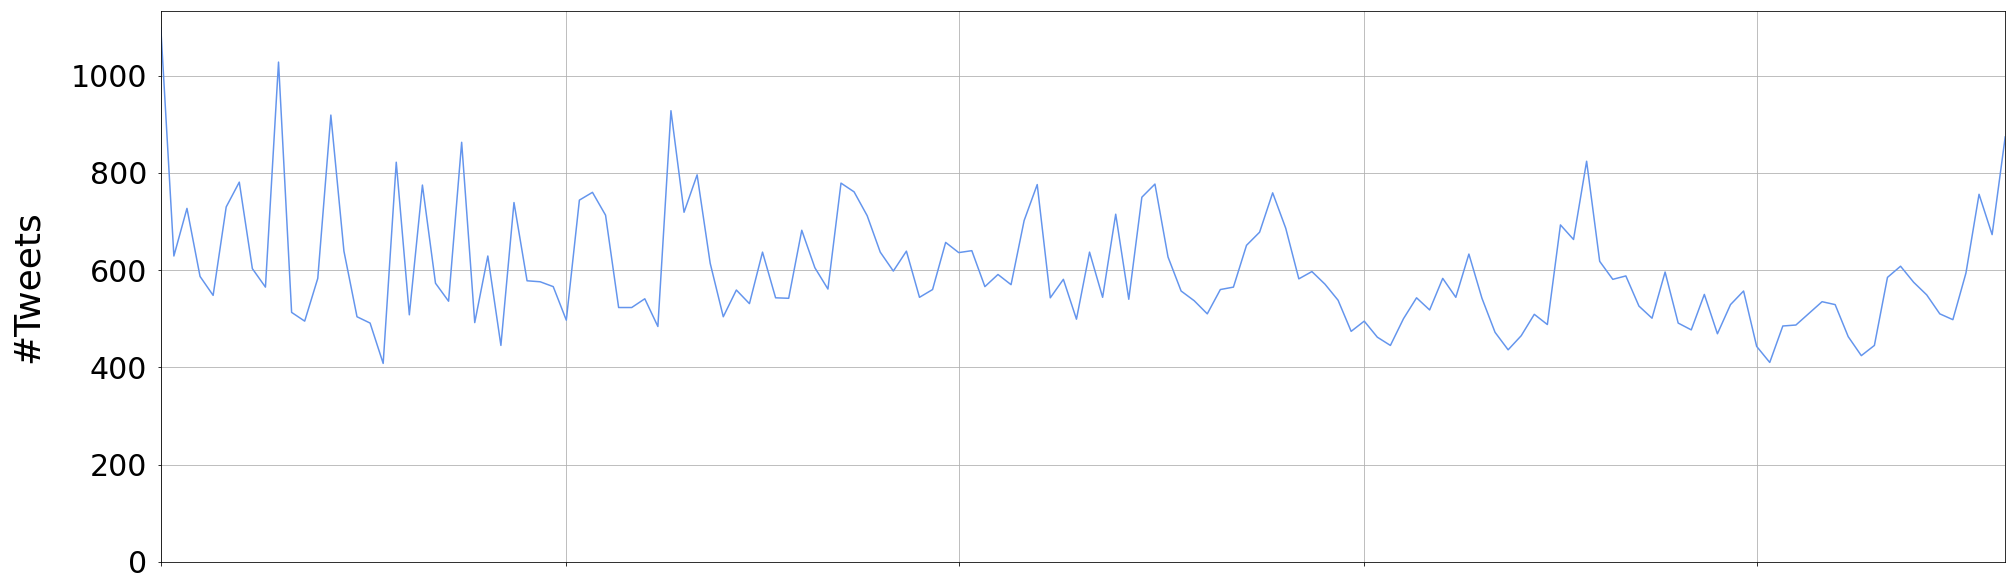
\includegraphics[width=1\textwidth]{images/monitoring/monitoring_lineplot_noX.png}
    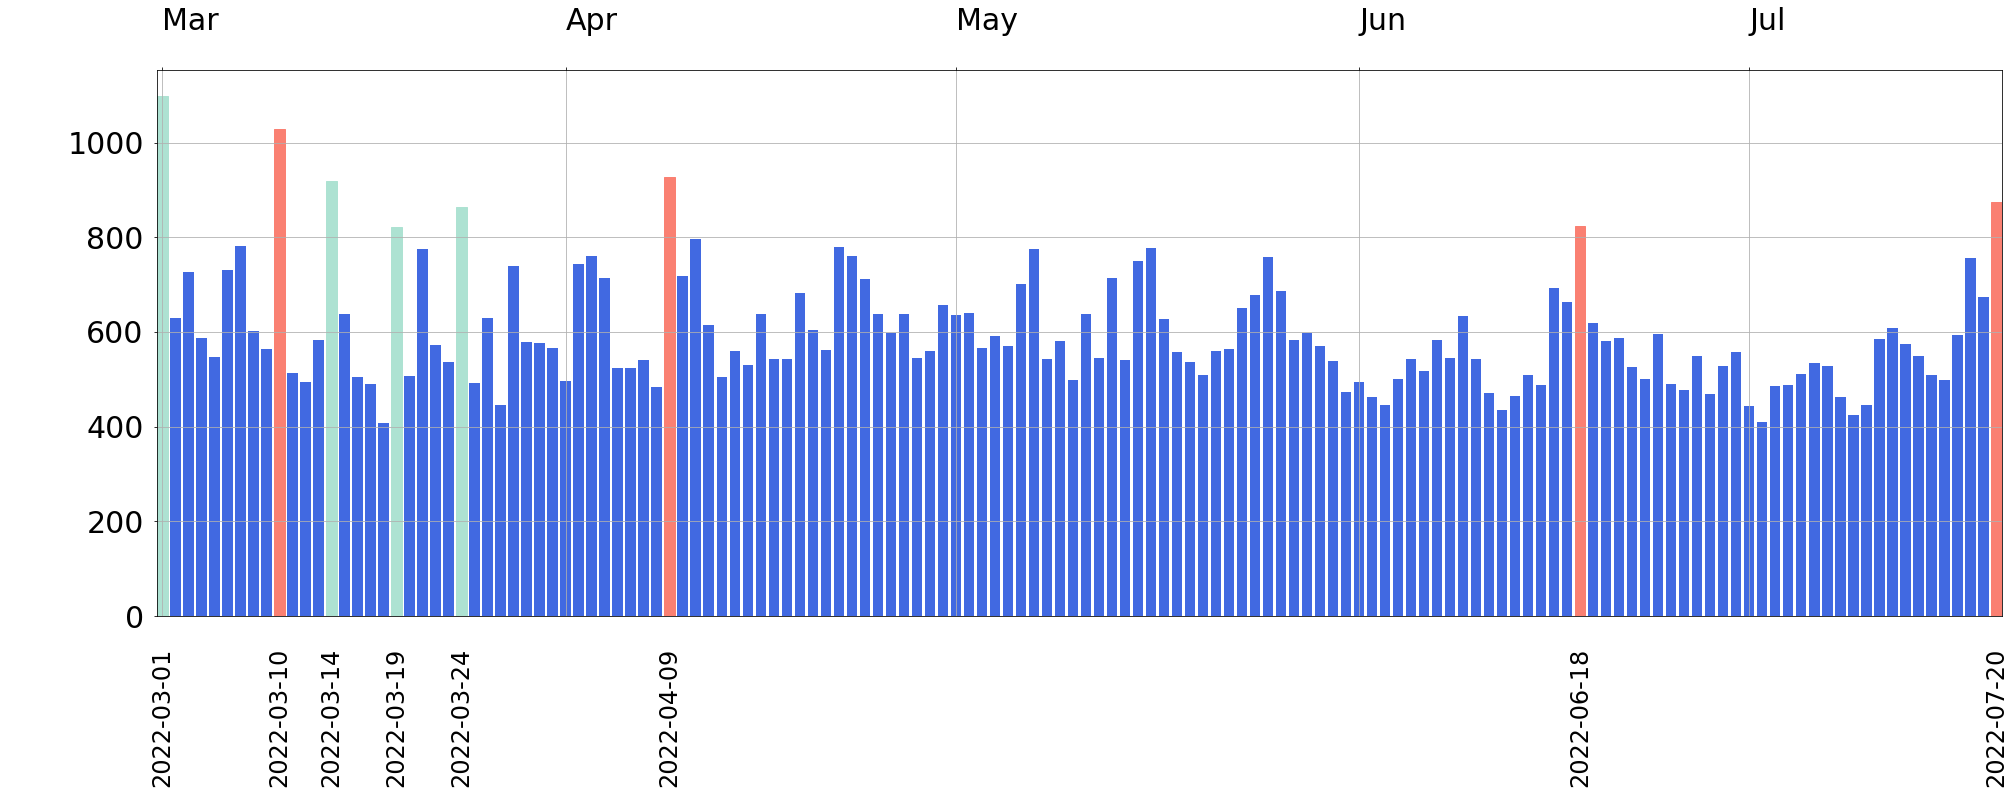
\includegraphics[width=1\textwidth]{images/monitoring/monitoring_barplot_peaks.png}
    \caption{Tweets distribution from 1st March, 2022 to 30th June, 2022} 
    \label{online-monitoring}
\end{figure}


\noindent
Table \ref{table:peaks} describes how many tweets have been collected in every temporal period and the hypothetical events that may have caused an increase in the volume of tweets posted.
\vspace{5mm}

\begin{table}[H]
\centering
\setlength{\tabcolsep}{5pt}
\renewcommand\arraystretch{1.5}
\begin{tabular}{cllp{6cm}r}
\hline
Name & Peak/Period & Date/Month & Event & Tweets \\
\hline
Period1 & Peak 1 & 2022-03-10 & Tv program GF semifinal & 1028 \\
Period2 & Peak 2 & 2022-04-09 & Episode of the tv program Amici with Sangiovanni as host  & 928  \\
Period3 &  May   & 2022-05    &    & 18959\\
Period4 & Peak 4 & 2022-06-18 & Vanessa Incontrada host of Gigi D'alessio's tv show & 824  \\
Period5 & Peak 5 & 2022-07-20 & Government crisis & 874\\
\hline
\end{tabular}
\caption{Peak/period details}
\label{table:peaks}
\end{table}

\vspace{5mm}
\vspace{5mm}
\subsection{Testing concept drift}

As suggested in \cite{greenpass} the 3 different types of concept drift that can be examinated are:

\begin{itemize}
    \item \textbf{static}, in which the model is always the same and it is tested using new tweets;
    \item \textbf{sliding window}, in which the model is retrained adding n new tweets and removing the older n ones;
    \item \textbf{incremental}, that retrains the model adding new labeled tweets also considering all the previous ones.
\end{itemize}

\noindent
For each event, except for the last one where only 60 tweets were taken, 80 tweets were randomly selected, manually labeled and used as test set for the \textbf{static model} to verify if the concept drift can really be a problem for this work.  

\vspace{5mm}
\begin{table}[H]
\centering
\setlength{\tabcolsep}{5pt}
\renewcommand\arraystretch{1.5}
\begin{tabular}{llc cc c cc c cc}
\hline
\multirow{2}*{Name} & \multirow{2}*{Peak} & \multirow{2}*{Accuracy (\%)} & \multicolumn{2}{c}{Precision (\%)} && \multicolumn{2}{c}{Recall (\%)} && \multicolumn{2}{c}{F1-score (\%)}\\
\cline{4-5} \cline{7-8} \cline{10-11}
\multicolumn{1}{c}{} &&& 0 & 1 && 0 & 1 && 0 & 1 \\
\hline
Period1 & Peak 1 & 73.75 & 74.35 & 73.17 && 72.50 & 75.00 && 73.41 & 74.07 \\
Period2 & Peak 2 & 72.50 & 70.45 & 75.00 && 77.50 & 67.50 && 73.80 & 71.05 \\
Period3 &  May   & 73.75 & 72.09 & 75.67 && 77.50 & 70.00 && 74.69 & 72.72 \\
Period4 & Peak 4 & 66.25 & 64.44 & 68.57 && 72.50 & 60.00 && 68.23 & 64.00 \\
Period5 & Peak 5 & 60.00 & 60.71 & 59.37 && 56.66 & 63.33 && 58.62 & 61.29 \\
\hline
\end{tabular}
\caption{Static model}
\label{table:static}
\end{table}
\noindent
For incremental and sliding approach, the training set have been updated basing on the behaviour of the different approaches. 

The \textbf{sliding approach} provides a new model for each new chunk of tweets, discarding the oldest and adding the newest, following the window dimension. The window dimension chosen was of 80 tweets (60 for July). For each peak, the new 80 (60) labeled tweets were inserted into the training set and the same number of the oldest tweets were removed. In this way, the number of tweets considered for the training set was always the same. The model is retrained each time considering the new tweets and the number of features changes during the various peaks. 


\vspace{5mm}
\begin{table}[H]
\centering
\setlength{\tabcolsep}{5pt}
\renewcommand\arraystretch{1.5}
\begin{tabular}{llc cc c cc c cc}
\hline
\multirow{2}*{Name} & \multirow{2}*{Peak} & \multirow{2}*{Accuracy (\%)} & \multicolumn{2}{c}{Precision (\%)} && \multicolumn{2}{c}{Recall (\%)} && \multicolumn{2}{c}{F1-score (\%)}\\
\cline{4-5} \cline{7-8} \cline{10-11}
\multicolumn{1}{c}{} &&& 0 & 1 && 0 & 1 && 0 & 1 \\
\hline
Period1 & Peak 1 & 73.75 & 72.09 & 75.67 && 77.50 & 70.00 && 74.69 & 72.72 \\
Period2 & Peak 2 & 76.25 & 70.58 & 86.20 && 90.00 & 62.50 && 79.12 & 72.46 \\
Period3 & May    & 71.25 & 68.08 & 75.75 && 80.00 & 62.50 && 73.56 & 68.49 \\
Period4 & Peak 4 & 71.25 & 69.76 & 72.97 && 75.00 & 67.50 && 72.28 & 70.12 \\
Period5 & Peak 5 & 63.33 & 64.28 & 62.50 && 60.00 & 66.66 && 62.06 & 64.51 \\
\hline
\end{tabular}
\caption{Sliding model}
\label{table:sliding}
\end{table}

\noindent
The \textbf{incremental approach} foresees a new retrain of the model each time basing on a training set gradually incremented with the previous examples. The approach adopted is not purely incremental but it is an approach that re-evaluates the model at every new peak. At each peak the training set have been incremented using the tweets of the previous peaks. In this way, at the end, the dimension of the training set goes from 1576 to 2132. With this approach, as consequence of the increasing of the training set dimension, the number of features increases too. 

\vspace{5mm}
\begin{table}[H]
\centering
\setlength{\tabcolsep}{5pt}
\renewcommand\arraystretch{1.5}
\begin{tabular}{llc cc c cc c cc}
\hline
\multirow{2}*{Name} & \multirow{2}*{Peak} & \multirow{2}*{Accuracy (\%)} & \multicolumn{2}{c}{Precision (\%)} && \multicolumn{2}{c}{Recall (\%)} && \multicolumn{2}{c}{F1-score (\%)}\\
\cline{4-5} \cline{7-8} \cline{10-11}
\multicolumn{1}{c}{} &&& 0 & 1 && 0 & 1 && 0 & 1 \\
\hline
Period1 & Peak 1 & 71.25 & 68.88 & 74.28 && 77.50 & 65.00 && 74.94 & 69.33 \\
Period2 & Peak 2 & 73.75 & 69.38 & 80.64 && 85.00 & 62.50 && 76.40 & 70.42 \\
Period3 & May    & 72.50 & 70.45 & 75.00 && 77.50 & 67.50 && 73.80 & 71.05 \\
Period4 & Peak 4 & 70.00 & 69.04 & 71.05 && 72.50 & 67.50 && 70.73 & 69.23 \\
Period5 & Peak 5 & 66.66 & 65.62 & 67.85 && 70.00 & 63.33 && 67.74 & 65.51 \\
\hline
\end{tabular}
\caption{Incremental model}
\label{table:incrementa}
\end{table}

\noindent
As it is possible to observe in the (Figure \ref{online-monitoring-accuracy}), the more time goes on the more the model designed with the static approach does not perform well. The other two, indeed, perform better during the time. Moreover, it is possible to observe that the static model has decreasing performances during the peaks but performs not so bad in May in which there is no event. The sliding, however, performs better than the incremental during all the peaks except for May and the last peak. 

\begin{figure}[H]
    \centering
    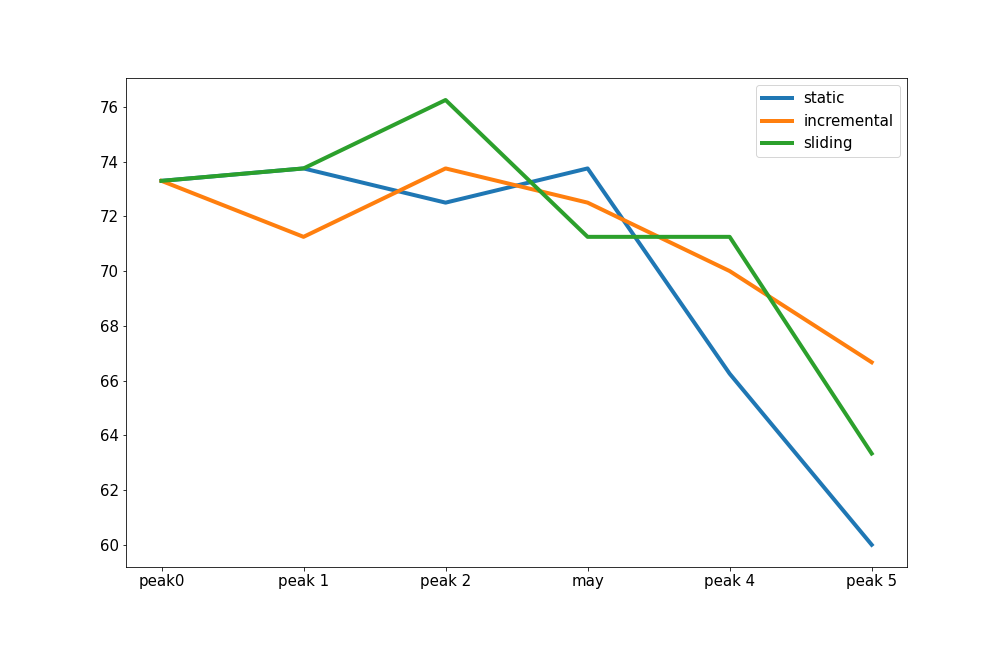
\includegraphics[width= 1\textwidth]{images/monitoring/accuracy_for_model.png}
    \caption{Accuracy for the three approaches} 
    \label{online-monitoring-accuracy}
\end{figure}

\noindent
The sliding approach results the one with the best performance except for the last peak. At the same time, the number of features of the incremental model increases quickly. On the contrary, the number of features using the sliding approach are always very low. 

\begin{figure}[H]
    \centering
    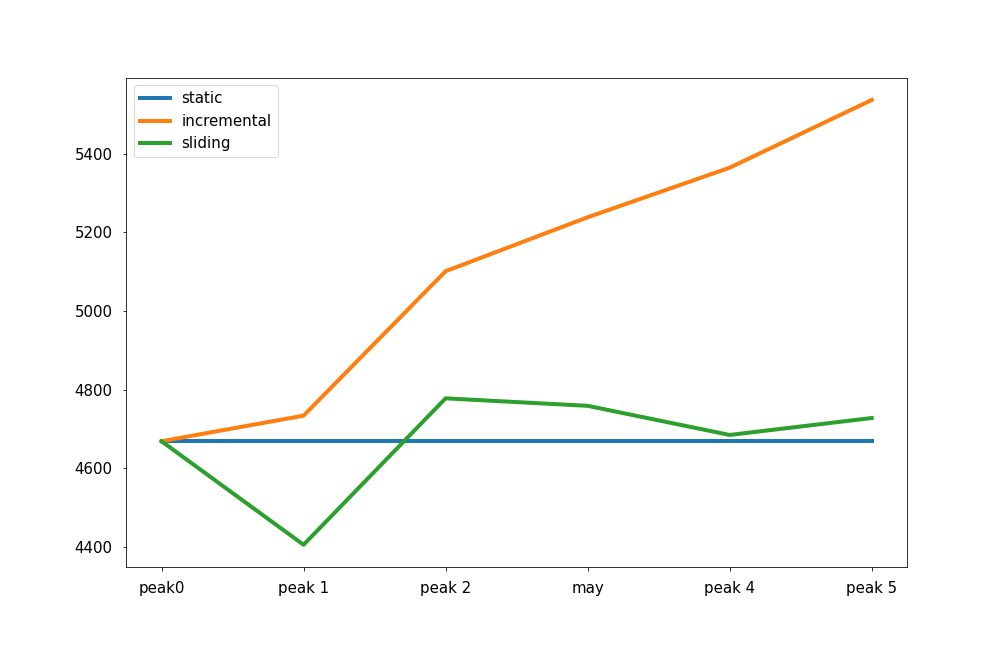
\includegraphics[width= 1\textwidth]{images/monitoring/features_for_model.png}
    \caption{Number of features for each approach} 
    \label{online-monitoring-features}
\end{figure}

\noindent
At the end, the sliding approach have been chosen. Indeed, the performance with this approach are mostly the best in the peaks and at the same time the number of features is low. However, in the last peak its performances decrease quickly and, for this reason, there is the possibility that in a long period the incremental approach will be more suitable than the sliding. The decrease in performance could be due to the fact that all the precedent peaks concern television programs events whereas, the last one, concerns a political event. It is possible that, considering an additional time period, the incremental approach will reveal to be the best choice.  

